%%%%%%%%%%%%%%%%%%%%%%%%%%%%%%%%%%%%%%%%%%%%%%%%%%%%%%%%%%%%%%%%%%%%%%%%%%%%%%%%
%Tutorial slides on Python.
%
% Author: Prabhu Ramachandran <prabhu at aero.iitb.ac.in>
% Copyright (c) 2005-2009, Prabhu Ramachandran
%%%%%%%%%%%%%%%%%%%%%%%%%%%%%%%%%%%%%%%%%%%%%%%%%%%%%%%%%%%%%%%%%%%%%%%%%%%%%%%%

\documentclass[14pt,compress]{beamer}
%\documentclass[draft]{beamer}
%\documentclass[compress,handout]{beamer}
%\usepackage{pgfpages} 
%\pgfpagesuselayout{2 on 1}[a4paper,border shrink=5mm]

% Modified from: generic-ornate-15min-45min.de.tex
\mode<presentation>
{
  \usetheme{Warsaw}
  \useoutertheme{infolines}
  \setbeamercovered{transparent}
}

\usepackage[english]{babel}
\usepackage[latin1]{inputenc}
%\usepackage{times}
\usepackage[T1]{fontenc}

% Taken from Fernando's slides.
\usepackage{ae,aecompl}
\usepackage{mathpazo,courier,euler}
\usepackage[scaled=.95]{helvet}

\definecolor{darkgreen}{rgb}{0,0.5,0}

\usepackage{listings}
\lstset{language=Python,
    basicstyle=\ttfamily\bfseries,
    commentstyle=\color{red}\itshape,
  stringstyle=\color{darkgreen},
  showstringspaces=false,
  keywordstyle=\color{blue}\bfseries}

%%%%%%%%%%%%%%%%%%%%%%%%%%%%%%%%%%%%%%%%%%%%%%%%%%%%%%%%%%%%%%%%%%%%%%
% Macros
\setbeamercolor{emphbar}{bg=blue!20, fg=black}
\newcommand{\emphbar}[1]
{\begin{beamercolorbox}[rounded=true]{emphbar} 
      {#1}
 \end{beamercolorbox}
}
\newcounter{time}
\setcounter{time}{0}
\newcommand{\inctime}[1]{\addtocounter{time}{#1}{\tiny \thetime\ m}}

\newcommand{\typ}[1]{\texttt{#1}}

\newcommand{\kwrd}[1]{ \texttt{\textbf{\color{blue}{#1}}}  }

%%% This is from Fernando's setup.
% \usepackage{color}
% \definecolor{orange}{cmyk}{0,0.4,0.8,0.2}
% % Use and configure listings package for nicely formatted code
% \usepackage{listings}
% \lstset{
%    language=Python,
%    basicstyle=\small\ttfamily,
%    commentstyle=\ttfamily\color{blue},
%    stringstyle=\ttfamily\color{orange},
%    showstringspaces=false,
%    breaklines=true,
%    postbreak = \space\dots
% }


%%%%%%%%%%%%%%%%%%%%%%%%%%%%%%%%%%%%%%%%%%%%%%%%%%%%%%%%%%%%%%%%%%%%%%
% Title page
\title[Exercises]{Exercises}

\author[FOSSEE] {FOSSEE}

\institute[IIT Bombay] {Department of Aerospace Engineering\\IIT Bombay}
\date[] {08 March, 2010\\Day 1, Session 5}
%%%%%%%%%%%%%%%%%%%%%%%%%%%%%%%%%%%%%%%%%%%%%%%%%%%%%%%%%%%%%%%%%%%%%%

%\pgfdeclareimage[height=0.75cm]{iitmlogo}{iitmlogo}
%\logo{\pgfuseimage{iitmlogo}}


%% Delete this, if you do not want the table of contents to pop up at
%% the beginning of each subsection:
\AtBeginSubsection[]
{
  \begin{frame}<beamer>
    \frametitle{Outline}
    \tableofcontents[currentsection,currentsubsection]
  \end{frame}
}


% If you wish to uncover everything in a step-wise fashion, uncomment
% the following command: 
%\beamerdefaultoverlayspecification{<+->}

%\includeonlyframes{current,current1,current2,current3,current4,current5,current6}

%%%%%%%%%%%%%%%%%%%%%%%%%%%%%%%%%%%%%%%%%%%%%%%%%%%%%%%%%%%%%%%%%%%%%%
% DOCUMENT STARTS
\begin{document}

\begin{frame}
  \titlepage
\end{frame}


\begin{frame}[fragile]
  \frametitle{Problem 1}
  \begin{columns}
    \column{0.5\textwidth}
    \hspace*{-0.5in}
    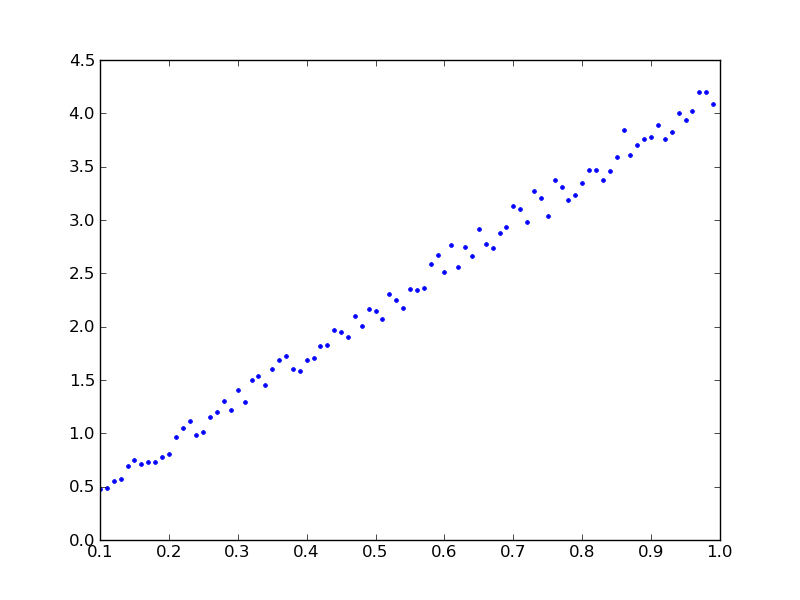
\includegraphics[height=2in, interpolate=true]{data/L-Tsq.png}
    \column{0.45\textwidth}
    \begin{block}{Example code}
    \tiny
    \begin{lstlisting}
l = []
t = []
for line in open('pendulum.txt'):
    point = line.split()
    l.append(float(point[0]))
    t.append(float(point[1]))
plot(l, t, '.')
    \end{lstlisting}
    \end{block}
  \end{columns}
  \begin{block}{Problem Statement}
    Tweak above code to plot data in file `pos.txt'.
  \end{block}
\end{frame}

\begin{frame}
  \frametitle{Problem 1 cont...}
  \begin{itemize}
  \item Label both the axes.
  \item What kind of motion is this?
  \item Title the graph accordingly.
  \item Annotate the position where vertical velocity is zero.
  \end{itemize}
\end{frame}

\begin{frame}[fragile]
  \frametitle{Problem 2}
  \begin{columns}
    \column{0.5\textwidth}
    \hspace*{-0.5in}
    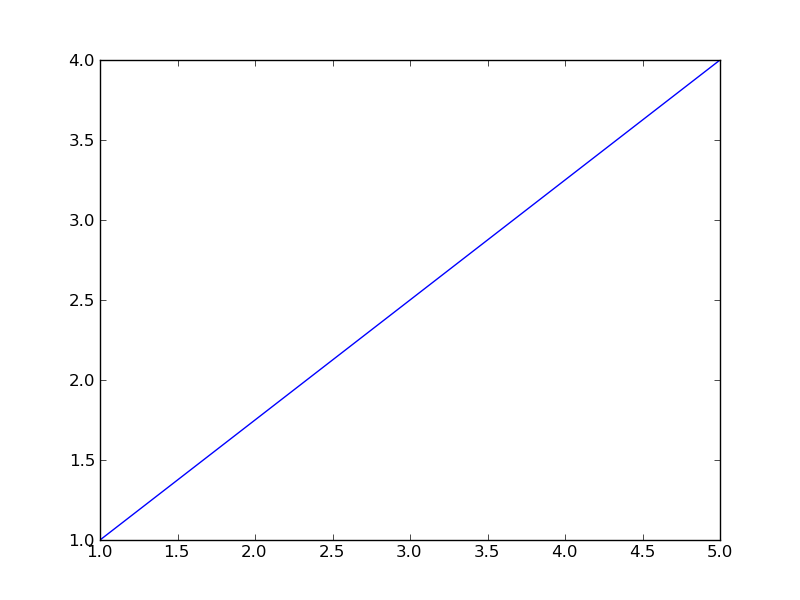
\includegraphics[height=2in, interpolate=true]{data/points}
    \column{0.45\textwidth}
    \begin{block}{Line between two points}
    \tiny
    \begin{lstlisting}
In []: x = [1, 5]
In []: y = [1, 4]
In []: plot(x, y)
    \end{lstlisting}
    \end{block}
  \end{columns}
  Line can be plotted using arrays of coordinates.
  \pause
  \begin{block}{Problem statement}
    Write a Program that plots a regular n-gon(Let n = 5).
  \end{block}  
\end{frame}


\begin{frame}[fragile]
  \frametitle{Problem 3}
  \begin{columns}
    \column{0.5\textwidth}
    \hspace*{-0.5in}
    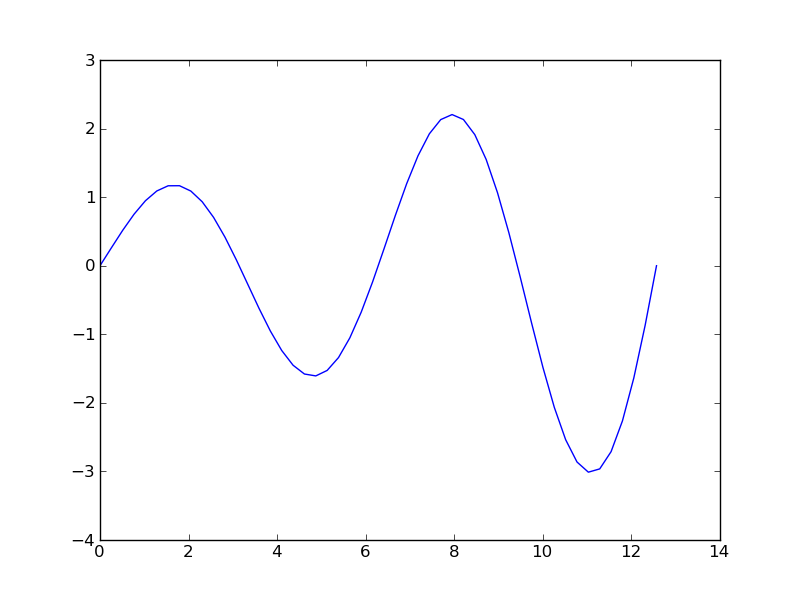
\includegraphics[height=2in, interpolate=true]{data/damp}
    \column{0.45\textwidth}
    \begin{block}{Damped Oscillation}
    \tiny
    \begin{lstlisting}
In []: x = linspace(0, 4*pi)
In []: plot(x, exp(x/10)*sin(x))
    \end{lstlisting}
    \end{block}
  \end{columns}
\end{frame}

\begin{frame}[fragile]
  \frametitle{Problem 3 cont...}
Create a sequence of images in which the damped oscillator($e^{-x/10}sin(x)$) slowly evolves over time.
\begin{columns}
\column{0.35\textwidth}
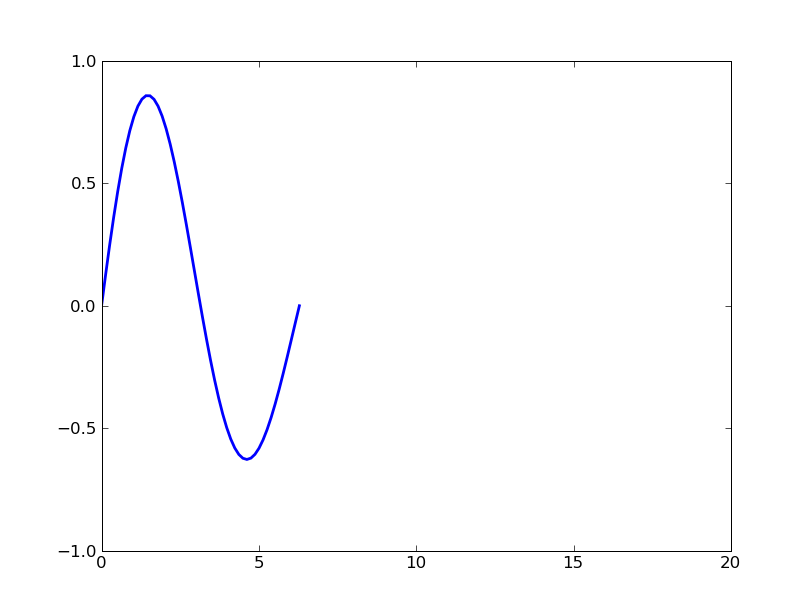
\includegraphics[width=1.5in,height=1.5in, interpolate=true]{data/plot2}
\column{0.35\textwidth}
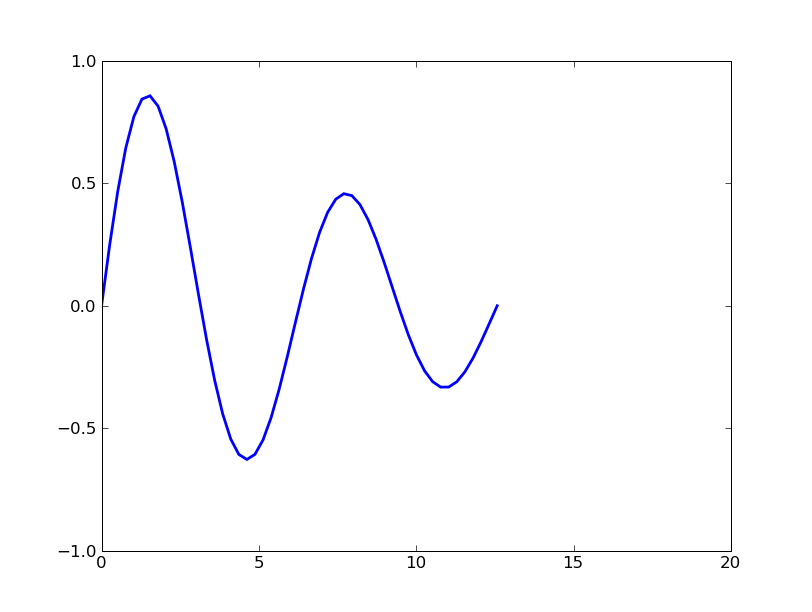
\includegraphics[width=1.5in,height=1.5in, interpolate=true]{data/plot4}
\column{0.35\textwidth}
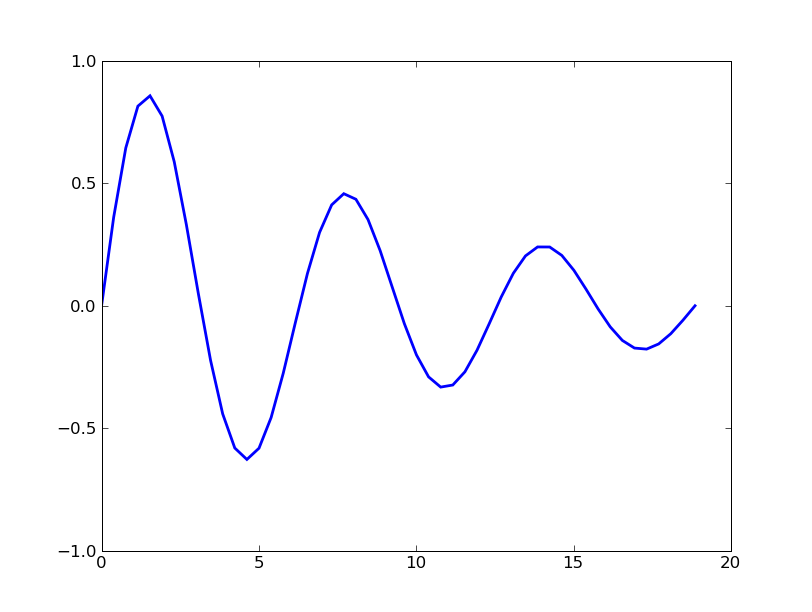
\includegraphics[width=1.5in,height=1.5in, interpolate=true]{data/plot6}
\end{columns}
\begin{block}{Hint}
\small
  \begin{lstlisting}
savefig('plot'+str(i)+'.png') #i is int variable  
  \end{lstlisting}  
\end{block}
\end{frame}

\begin{frame}[fragile]
  \frametitle{Problem 4}
  \begin{lstlisting}
In []: x = imread('smoothing.png')
In []: x.shape
Out[]: (256, 256)
In []: imshow(x,cmap=cm.gray)
  \end{lstlisting}
\emphbar{Replace each pixel with mean of neighboring pixels}
  \begin{center}
  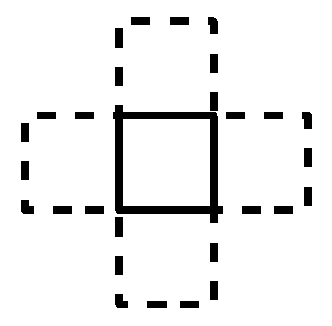
\includegraphics[height=1in, interpolate=true]{data/neighbour}
  \end{center}
\end{frame}

\begin{frame}
  \begin{center}
    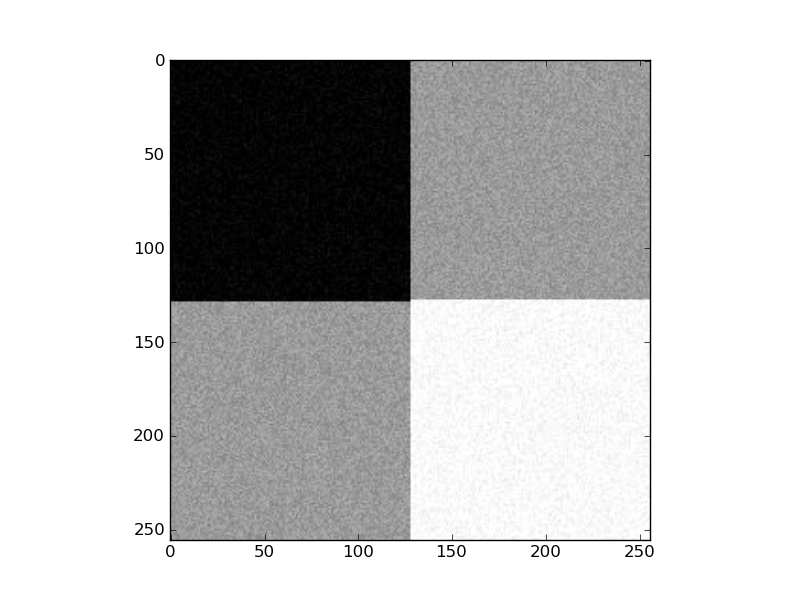
\includegraphics[height=3in, interpolate=true]{data/smoothing}    
  \end{center}
\end{frame}

\begin{frame}[fragile]
  \frametitle{Problem 4: Approach}
  For \typ{y} being resultant image:
  \begin{lstlisting}
y[1, 1] = x[0, 1]/4 + x[1, 0]/4 
          + x[2, 1]/4 + x[1, 2]/4    
  \end{lstlisting}
   \begin{columns}
    \column{0.45\textwidth}
    \hspace*{-0.5in}
    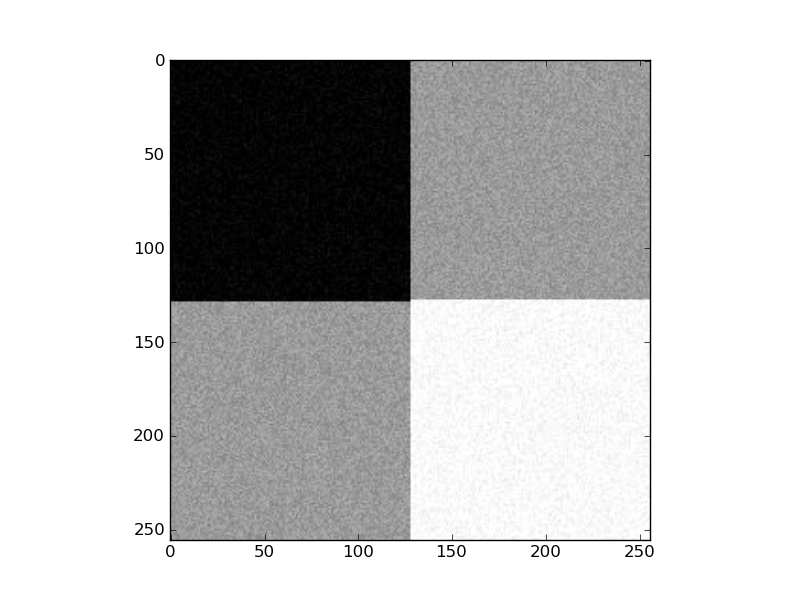
\includegraphics[height=1.5in, interpolate=true]{data/smoothing}
    \column{0.45\textwidth}
    \hspace*{-0.5in}
    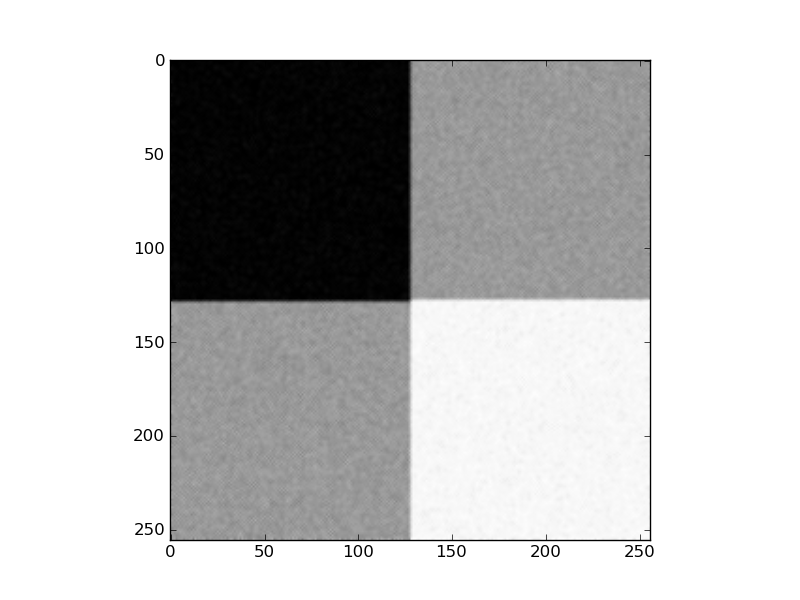
\includegraphics[height=1.5in, interpolate=true]{data/after-filter}
  \end{columns}
   \begin{block}{Hint:}
     Use array Slicing.
   \end{block}
\end{frame}

\begin{frame}[fragile]
  \frametitle{Solution}
  \begin{lstlisting}
In []: y = zeros_like(x)
In []: y[1:-1,1:-1] = x[:-2,1:-1]/4+
                      x[2:,1:-1]/4+
                      x[1:-1,2:]/4+
                      x[1:-1,:-2]/4
In []: imshow(y,cmap=cm.gray)
  \end{lstlisting}
\end{frame}


\end{document}

%% \begin{frame}
%%   \frametitle{Problem 4}
%%   Legendre polynomials $P_n(x)$ are defined by the following recurrence relation

%% \center{$(n+1)P_{n+1}(x) - (2n+1)xP_n(x) + nP_{n-1}(x) = 0$}\\

%% with $P_0(x) = 1$, $P_1(x) = x$ and $P_2(x) = (3x^2 - 1)/2$. Compute the next three 
%%    Legendre polynomials and plot all 6 over the interval [-1,1].
%% \end{frame}

%% \begin{frame}[fragile] 
%% \frametitle{Problem Set 5}
%%   \begin{columns}
%%     \column{0.6\textwidth}
%%     \small{
%%     \begin{itemize}
%%       \item[3] Consider the iteration $x_{n+1} = f(x_n)$ where $f(x) = kx(1-x)$.  Plot the successive iterates of this process as explained below. 
%%     \end{itemize}}
%%     \column{0.35\textwidth}
%%     \hspace*{-0.5in}
%%   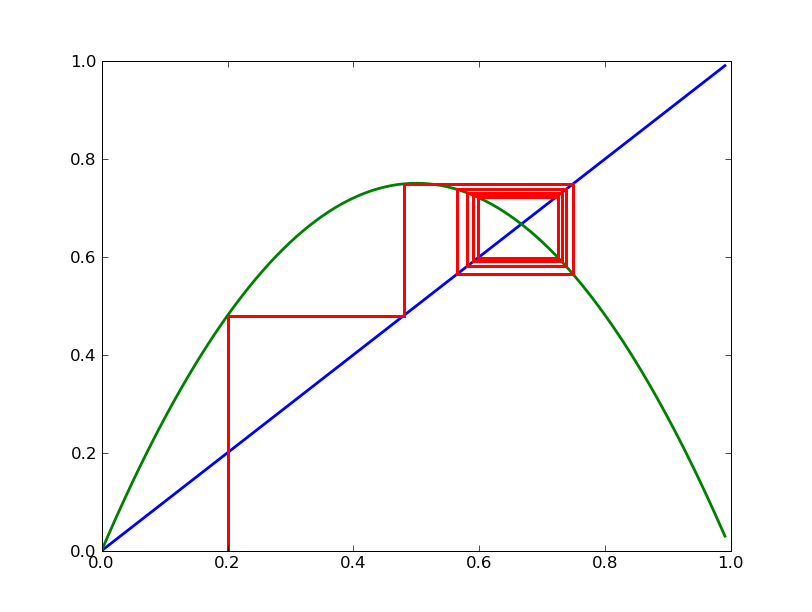
\includegraphics[height=1.6in, interpolate=true]{data/cobweb}  
%% \end{columns}
%% \end{frame}

%% \begin{frame}
%%   \frametitle{Problem Set 5.3}
%%   Plot the cobweb plot as follows:
%%   \begin{enumerate}
%%     \item Start at $(x_0, 0)$ ($\implies$ i=0)
%%     \item Draw a line to $(x_i, f(x_i))$
%%     \item Set $x_{i+1} = f(x_i)$
%%     \item Draw a line to $(x_{i+1}, x_{i+1})$
%%     \item $(i\implies i+1)$ 
%%     \item Repeat from 2 for as long as you want 
%%   \end{enumerate}
%% \inctime{20}
%% \end{frame}
